\let\lesson\undefined
\newcommand{\lesson}{\phantomlesson{Bài 10.}}
\setcounter{section}{2}
\section{Bài tập trắc nghiệm}
\begin{enumerate}[label=\bfseries Câu \arabic*:,leftmargin=1.5cm]
	\item \mkstar{1}\\
	{Đại lượng đặc trưng cho mức quán tính của một vật là
		\begin{mcq}(4)
			\item trọng lượng.
			\item khối lượng.
			\item vận tốc.
			\item lực.
		\end{mcq}
	
}
\hideall{
\textbf{Đáp án: B.}
}

\item \mkstar{1}\\
Biểu thức nào sau đây là biểu thức của định luật II Newton khi vật có khối lượng không đổi trong quá trình xem xét?
\begin{mcq}(4)
	\item $\vec{a}=\dfrac{\vec{F}}{m}$.
	\item $F=m\cdot a$.
	\item $a=\dfrac{v-v_0}{t-t_0}$.
	\item $\vec{a}=\dfrac{\vec{v}-\vec{v}_0}{t-t_0}$.
\end{mcq}
\hideall{
\textbf{Đáp án A.}
}

\item \mkstar{1}\\
 Đơn vị đo lực newton được viết theo các đơn vị cơ bản trong hệ SI là
 \begin{mcq}(4)
 	\item $\si{\kilogram/\meter^2}$.
 	\item $\si{\kilogram/\second^2}$.
 	\item $\si{\kilogram\cdot\meter^2/\second}$.
 	\item $\si{\kilogram\cdot\meter/\second^2}.$
 \end{mcq}
\hideall{
\textbf{Đáp án D.}
}

\item \mkstar{2}\\
Khi nói về một vật chịu tác dụng của lực, phát biểu nào sau đây đúng?
\begin{mcq}
	\item Khi không có lực tác dụng, vật không thể chuyển động.
	\item Khi ngừng tác dụng lực lên vật, vật này sẽ dừng lại.
	\item Gia tốc của vật luôn cùng chiều với hợp lực tác dụng.
	\item Khi có lực tác dụng lên vật, vận tốc của vật tăng.
\end{mcq}
\hideall{
\textbf{Đáp án C.}
}

\item\mkstar{2}\\
{Trong chuyển động thẳng chậm dần đều thì hợp lực tác dụng vào vật
	\begin{mcq}
		\item cùng chiều với chuyển động.
		\item cùng chiều với chuyển động và có độ lớn không đổi.
		\item ngược chiều với chuyển động và có độ lớn nhỏ dần.
		\item ngược chiều với chuyển động và có độ lớn không đổi.
	\end{mcq}

}
\hideall{
\textbf{Đáp án: D.}
}

\item \mkstar{2}\\
Một vật đang chuyển động nhanh dần đều dưới tác dụng của lực kéo mà lực đó đột ngột giảm độ lớn thì
\begin{mcq}
	\item gia tốc của vật không đổi.
	\item gia tốc của vật giảm.
	\item gia tốc của vật tăng.
	\item gia tốc và vận tốc của vật đều giảm.
\end{mcq}
\hideall{
\textbf{Đáp án B.}\\
Vì độ lớn của gia tốc tỉ lệ với độ lớn của hợp lực tác dụng lên vật $a=\dfrac{F}{m}$ nên khi độ lớn lực kéo giảm thì độ lớn gia tốc giảm.
}

\item\mkstar{2}\\
{Nếu một vật đang chuyển động có gia tốc mà lực tác dụng lên vật tăng lên thì vật sẽ thu được gia tốc 
	\begin{mcq}(2)
		\item nhỏ hơn.
		\item lớn hơn.
		\item bằng 0.
		\item không đổi.
	\end{mcq}

}
\hideall{
\textbf{Đáp án: B.}
}

\item \mkstar{2}\\
{Hợp lực của tất cả các lực tác dụng lên vật
	\begin{mcq}
		\item có hướng trùng với hướng chuyển động của vật.
		\item có hướng không trùng với hướng chuyển động của vật.
		\item có hướng trùng với hướng của gia tốc mà vật thu được.
		\item khi vật chuyển động thẳng đều có độ lớn thay đổi.
	\end{mcq}

}
\hideall{
\textbf{Đáp án: C.}
}

\item \mkstar{2}\\
{Một người tiếp viên hàng không đang đẩy một chiếc xe đẩy xuống lối đi của một chiếc máy bay đang bay. Khi xác định gia tốc của xe đẩy so với máy bay thì ta không cần chú ý đến dữ kiện nào sau đây?   
	\begin{mcq}(2)
		\item Lực ma sát của bánh xe với mặt sàn.  
		\item Lực mà người tiếp viên tác dụng lên xe đẩy.  
		\item Vận tốc của máy bay.  
		\item Khối lượng của xe đẩy và hàng hoá trên đó. 
	\end{mcq}
	
}
\hideall{
	\textbf{Đáp án: C.}
}

\item \mkstar{2}\\
Những nhận định nào sau đây là đúng?
\begin{enumerate}[label=\arabic*.]
	\item Khi vật chịu tác dụng của lực $\vec{F}$ thì gia tốc $\vec{a}$ mà vật thu được cùng phương nhưng ngược chiều với $\vec{F}$.
	\item Khi vật chỉ chịu tác dụng của lực $\vec{F}$ thì gia tốc $\vec{a}$ mà vật thu được cùng hướng với $\vec{F}$.
	\item Khi vật chịu tác dụng của hai lực cân bằng thì gia tốc $\vec{a}$ của vật thu được khác không.
	\item Khi vật chịu tác dụng của nhiều lực thì gia tốc $\vec{a}$ của vật thu được cùng hướng với lực tổng hợp tác dụng lên vật.
\end{enumerate}
\begin{mcq}(4)
	\item 2, 4.
	\item 1, 3.
	\item 1, 4.
	\item 3, 4.
\end{mcq}
\hideall{
\textbf{Đáp án A.}
}

\item \mkstar{2}\\
Sau khoảng thời gian $\SI{0.02}{\second}$ tiếp xúc với chân của cầu thủ, quả bóng khối lượng $\SI{500}{\gram}$ ban đầu đứng yên bay đi với tốc độ $\SI{54.0}{\kilo\meter/\hour}$. Lực tác dụng lên quả bóng có độ lớn là
\begin{mcq}(4)
	\item $\SI{250}{\newton}$.
	\item $\SI{375}{\newton}$.
	\item $\SI{1.35}{\kilo\newton}$.
	\item $\SI{13.5}{\kilo\newton}$.
\end{mcq}
\hideall{
	\textbf{Đáp án B.}\\
	$v=\SI{54}{\kilo\meter/\hour}=\SI{15}{\meter/\second}$.\\
	Gia tốc quả bóng thu được:
	$$a=\dfrac{\Delta v}{\Delta t}=\SI{750}{\meter/\second^2}.$$
	Độ lớn lực tác dụng lên quả bóng:
	$$F=ma=\left(\SI{0.5}{\kilo\gram}\right)\cdot\left(\SI{750}{\newton/\meter^2}\right)=\SI{375}{\newton}.$$
}

\item \mkstar{2}\\
Một lực không đổi tác dụng vào một vật có khối lượng $\SI{7.5}{\kilogram}$ làm vật thay đổi tốc độ từ $\SI{8}{\meter/\second}$ đến $\SI{3}{\meter/\second}$ trong khoảng thời gian $\SI{2}{\second}$ nhưng vẫn giữ nguyên chiều chuyển động. Lực tác dụng vào vật có giá trị là
\begin{mcq}(4)
	\item $\SI{18.75}{\newton}$.
	\item $\SI{-18.75}{\newton}$.
	\item $\SI{20.5}{\newton}$.
	\item $\SI{-20.5}{\newton}$.
\end{mcq}
\hideall{
\textbf{Đáp án B.}\\
Lực tác dụng vào vật có giá trị:
$$F=ma=m\cdot\dfrac{\Delta v}{\Delta t}=\SI{-18.75}{\newton}.$$
}

\item \mkstar{3}\\
Một xe tải chờ đầy hàng và một xe con đang chuyển động cùng tốc độ mà muốn dừng lại cùng lúc thì lực hãm tác dụng lên xe tải sẽ phải
\begin{mcq}
	\item nhỏ hơn lực hãm lên xe con.
	\item bằng lực hãm lên xe con.
	\item lớn hơn lực hãm lên xe con.
	\item có thể lớn hơn hoặc nhỏ hơn lực hãm lên xe con.
\end{mcq}
\hideall{
	\textbf{Đáp án C.}\\
	Ban đầu 2 xe chuyển động cùng tốc độ và muốn dừng lại cùng lúc thì gia tốc hãm phanh của hai xe là như nhau $a=\dfrac{\Delta v}{\Delta t}$.\\
	Độ lớn lực hãm lên mỗi xe $F=m\left|a\right|$. Vì khối lượng xe tải lớn hơn nhiều so với khối lượng xe con nên lực hãm tác dụng lên xe tải phải lớn hơn lực hãm lên xe con.
}

\item\mkstar{3}\\
{Một vật có khối lượng $\SI{2}{\kilogram}$ chuyển động thẳng nhanh dần đều từ trạng thái nghỉ. Vật đi được $\SI{100}{\centi\meter}$ trong $\SI{0.25}{\second}$. Gia tốc của vật và hợp lực tác dụng lên vật có giá trị lần lượt là
	\begin{mcq}(4)
		\item $\SI{32}{\meter/\second^2}$; $\SI{64}{\newton}$.
		\item $\SI{0.64}{\meter/\second^2}$; $\SI{1.2}{\newton}$.
		\item $\SI{6.4}{\meter/\second^2}$; $\SI{12.8}{\newton}$.
		\item $\SI{64}{\meter/\second^2}$; $\SI{128}{\newton}$.
	\end{mcq}

}
\hideall{
\textbf{Đáp án: A.}\\
Gia tốc của vật:
$$a=\dfrac{2s}{t^2}=\SI{32}{\meter/\second^2}$$
Hợp lực tác dụng lên vật:
$$F=ma=\SI{64}{\newton}.$$
}

\item\mkstar{3}\\
{Một quả bóng đang nằm yên trên  mặt đất thì bị một cầu thủ đá bằng một lực $\SI{13.5}{\newton}$ và bóng thu được gia tốc $\SI{6.5}{\meter/\second^2}$. Bỏ qua mọi ma sát. Khối lượng của bóng là
	\begin{mcq}(4)
		\item $\SI{2.08}{\kilogram}$.
		\item $\SI{0.5}{\kilogram}$.
		\item $\SI{0.8}{\kilogram}$.
		\item $\SI{5}{\kilogram}$.
	\end{mcq}

}
\hideall{
\textbf{Đáp án: A.}\\
Khối lượng của quả bóng:
$$m=\dfrac{F}{a}=\SI{2.08}{\kilogram}.$$
}

\item \mkstar{3}\\
{Lần lượt tác dụng lực có độ lớn $F_1$ và $F_2$ lên một vật khối lượng $m$, vật thu được gia tốc có độ lớn lần lượt là $a_1$ và $a_2$. Biết $1,5F_1=F_2$. Bỏ qua mọi ma sát. Tỉ số $\dfrac{a_2}{a_1}$ là
	\begin{mcq}(4)
		\item $\dfrac{3}{2}$.
		\item $\dfrac{2}{3}$.
		\item $3$.
		\item $\dfrac{1}{3}$.
	\end{mcq}

}
\hideall{
\textbf{Đáp án: A.}\\
$$\dfrac{a_2}{a_1}=\dfrac{F_2}{F_1}=\dfrac{3}{2}.$$
}

\item \mkstar{3}\\
{Một lực không đổi tác dụng vào một vật có khối lượng $\SI{2.5}{\kilogram}$ làm vận tốc của nó tăng dần từ $\SI{2}{\meter/\second}$ đến $\SI{6}{\meter/\second}$ trong $\SI{2}{\second}$. Lực tác dụng vào vật có độ lớn bằng 
	\begin{mcq}(4)
		\item $\SI{7.5}{\newton}$.
		\item $\SI{5}{\newton}$.
		\item $\SI{0.5}{\newton}$.
		\item $\SI{2.5}{\newton}$.
	\end{mcq}

}
\hideall{
\textbf{Đáp án: B.}\\
Gia tốc của vật:
$$a=\dfrac{v_2-v_1}{\Delta t}=\SI{2}{\meter/\second^2}$$
Lực tác dụng vào vật:
$$F=ma=\SI{5}{\newton}.$$
}

\item \mkstar{3}\\
Một mẫu siêu xe có khối lượng là 1,60 tấn. Nếu coi xe tăng tốc đều và lực trung bình để tăng tốc xe là $\SI{24.0}{\kilo\newton}$ thì mẫu xe này cần bao nhiêu lâu để có thể tăng tốc từ trạng thái nghỉ lên đến tốc độ $\SI{108}{\kilo\meter/\hour}$?
\begin{mcq}(2)
	\item Khoảng $\SI{2.00}{\second}$.
	\item Khoảng $\SI{7.20}{\second}$.
	\item Khoảng $\SI{10.0}{\second}$.
	\item Khoảng $\SI{15.0}{\second}$.
\end{mcq}
\hideall{
	\textbf{Đáp án A.}\\
	$v=\SI{108}{\kilo\meter/\hour}=\SI{30}{\meter/\second}.$\\
	Gia tốc xe thu được:
	$$a=\dfrac{F}{m}=\dfrac{\SI{24E3}{\newton}}{\SI{1.6E3}{\kilogram}}=\SI{15}{\meter/\second^2}.$$
	Thời gian để xe tăng tốc lên tốc độ $\SI{108}{\kilo\meter/\hour}$ từ trạng thái đứng yên:
	$$\Delta t=\dfrac{\Delta v}{a}=\dfrac{\SI{30}{\meter/\second}-\SI{0}{\meter/\second}}{\SI{15}{\meter/\second^2}}=\SI{2}{\second}.$$}

\item \mkstar{3}\\
{Một hợp lực $\SI{2}{\newton}$ tác dụng vào một vật có khối lượng $\SI{2}{\kilogram}$ lúc đầu đứng yên, trong khoảng thời gian $\SI{2}{\second}$. Đoạn đường mà vật đó đi được trong khoảng thời gian đó là
\begin{mcq}(4)
	\item $\SI{8}{\meter}$.
	\item $\SI{2}{\meter}$.
	\item $\SI{1}{\meter}$.
	\item $\SI{4}{\meter}$.
\end{mcq}
}
\hideall{
\textbf{Đáp án: B.}\\
Gia tốc vật thu được:
$$a=\dfrac{F}{m}=\SI{1}{\meter/\second^2}$$
Đoạn đường vật đi được trong khoảng thời gian $\SI{2}{\second}$:
$$s=\dfrac{1}{2}\cdot at^2=\SI{2}{\meter}.$$
}

\item \mkstar{3}\\
{Một ô tô khối lượng 1 tấn đang chuyển động với tốc độ $\SI{72}{\kilo\meter/\hour}$ thì hãm phanh chuyển động thẳng chậm dần đều và đi thêm được $\SI{500}{\meter}$ rồi dừng lại. Chọn chiều dương là chiều chuyển động. Lực hãm tác dụng lên xe là
	\begin{mcq}(4)
		\item $\SI{800}{\newton}$.
		\item $\SI{-800}{\newton}$.
		\item $\SI{400}{\newton}$.
		\item $\SI{-400}{\newton}$.
	\end{mcq}

}
\hideall{
\textbf{Đáp án: D.}\\
Gia tốc của xe trong quá trình hãm phanh:
$$a=-\dfrac{v^2_0}{2s}=\SI{-0.4}{\meter/\second^2}$$
Lực hãm tác dụng lên xe:
$$F_h=ma=\SI{-400}{\newton}.$$
}

\end{enumerate}
\section{Bài tập tự luận}
\begin{enumerate}[label=\bfseries Bài \arabic*:,leftmargin=1.5cm]
	\item \mkstar{1}\\
	Hãy giải thích tại sao để đặt được cùng một vận tốc từ trạng thái đứng yên, xe có khối lượng càng lớn sẽ tốn nhiều thời gian để tăng tốc hơn nếu lực kéo của động cơ là như nhau đối với các xe đang xét.
	\hideall{
Dựa vào công thức định luật II Newton, độ lớn gia tốc vật thu được $a=\dfrac{F}{m}$. Với cùng một lực thì vật có khối lượng càng lớn sẽ có gia tốc càng nhỏ nên có sự thay đổi vận tốc chậm hơn.
}
	\item \mkstar{2}
	
	
	{Cho đồ thị biểu diễn mối liên hệ giữa các lực tác dụng lên một vật và gia tốc gây ra tương ứng. Khối lượng của vật là bao nhiêu?
		
		\begin{center}
			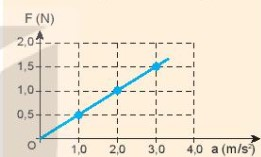
\includegraphics[scale=1]{../figs/VN10-2022-PH-TP017-2.jpg}
		\end{center}
	}
	
	\hideall
	{	
		
		Khối lượng của vật là
		
		$$m = \dfrac{F_1}{a_1} = \dfrac{F_2}{a_2} = \dfrac{F_3}{a_2} = \dfrac{\text{0,5}}{\text{1,0}} = \dfrac{\text{1,0}}{\text{2,0}} =\dfrac{\text{1,5}}{\text{3,0}} = \SI{0,5}{kg}.$$
		
	}

	\item \mkstar{2}
	
	{
		
		Một lực có độ lớn $\SI{6}{N}$ tác dụng lên vật có khối lượng $\SI{0,5}{kg}$ đang đứng yên. Bỏ qua ma sát và các lực cản. Gia tốc của vật bằng bao nhiêu?
		
	}
	
	\hideall{
		
		Gia tốc của vật là:
		
		$$a = \dfrac{F}{m} = \SI{12}{m/s}^2.$$
	}



	\item \mkstar{3}
	
	{
		Xét một ô tô có khối lượng $\SI{900}{kg}$ đang đi với vận tốc $\SI{20}{m/s}$ thì người lái xe nhìn thấy đèn giao thông chuyển màu đỏ ở phía trước. Để xe giảm tốc độ và dừng lại sau $\SI{10}{s}$ thì lực hãm khi phanh ô tô phải là bao nhiêu?
	}
	
	\hideall{
		Chọn chiều dương cùng chiều chuyển động ban đầu của xe.\\
		Gia tốc của ô tô cần có để giảm tốc và dừng lại là:
		$$a = \dfrac{\Delta v}{\Delta t} = -\SI{2}{m/s}^2.$$
		Lực hãm phanh:
		$$F = ma = - \text{1,8} \cdot 10^3\ \text{N}.$$
		Như vậy, độ lớn lực hãm khi phanh là $\text{1,8}\cdot 10^3\ \text{N}$ để xe giảm tốc và dừng lại sau $\SI{10}{s}$ từ vận tốc $\SI{20}{m/s}$. Dấu "-" thể hiện lực ngược hướng chuyển động ban đầu của xe.
	}
	
	\item \mkstar{3}
	
	{
		
		Mẫu xe điện có thời gian tăng tốc nhanh nhất được thử nghiệm đã tăng tốc từ $\SI{0}{km/h}$ đến $\SI{97}{km/h}$ trong 1,98 giây. Hãy tính gia tốc của xe và lực để tạo ra gia tốc đó. Coi xe chuyển động biến đổi đều và khối lượng của mẫu xe này là 2 tấn.
	}
	
	\hideall{
		
		Đổi $\SI{97}{km/h} = \SI{26,94}{m/s}.$\\
		Gia tốc của xe trong quá trình tăng tốc:
		$$a = \dfrac{v - v_0}{t} = \SI{13,61}{m/s}^2.$$
		Độ lớn lực để tạo ra gia tốc trên:
		$$F = ma = \SI{27220}{\newton}$$
	}





	\item \mkstar{3}
	
	{
		
		Thông số mẫu xe ô tô được cung cấp như bảng dưới đây. Tính lực tác dụng để mẫu xe trên chở đủ tải trọng và tăng tốc từ trạng thái nghỉ đến tốc độ tối ưu trong 2 giây.
		
		\begin{center}
			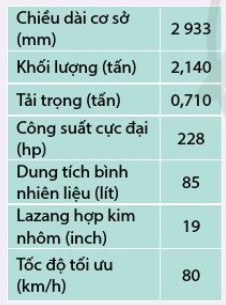
\includegraphics[scale=1]{../figs/VN10-2022-PH-TP016-1.jpg}
		\end{center}
		
	}
	
	\hideall{
		
		Để xe trên chở đủ tải trọng và tăng tốc từ trạng thái nghỉ đến tốc độ tối ưu trên 2 giây thì gia tốc của xe là:
		
		$$a = \dfrac{v - v_0}{t} = \SI{11,11}{m/s}^2.$$
		
		Lực tác dụng là
		
		$$F = ma= \SI{31666.6}{\newton}.$$
	}
	\item \mkstar{3}
	
	{
		
		Một người có khối lượng $\SI{60}{kg}$ đi trên xe đạp có khối lượng $\SI{20}{kg}$. Khi xuất phát, hợp lực tác dụng lên xe đạp là $\SI{200}{N}$. Giả sử hợp lực tác dụng lên xe đạp không đổi, hãy tính vận tốc của xe đạp sau $\SI{5}{s}$.
	}
	
	\hideall{
		
		Xe đạp đi với gia tốc là:
		
		$$a=\dfrac{F}{m}= \SI{2,5}{m/s}^2.$$
		
		Vận tốc của xe đạp sau $\SI{5,00}{s}$ là:
		
		$$v=v_0+at = \SI{12,5}{m/s}.$$
		
	}
	
	\item \mkstar{3}
	
	{
		
		Một ô tô có khối lượng 1 tấn đang chuyển động với $v = \SI{54}{km/h}$ thì tắt máy, hãm phanh, chuyển động chậm dần đều. Biết độ lớn lực hãm $\SI{3000}{N}$. Xác định quãng đường xe đi được cho đến khi dừng lại.
	}
	
	\hideall{
		
		Chọn chiều dương cùng chiều chuyển động của ô tô.\\
		Gia tốc của ô tô trong quá trình hãm phanh:
		$$a = \dfrac{-F}{m} = -\SI{3}{m/s}^2.$$
		Khi ô tô dừng ta có $v=0$, quãng đường ô tô đi được cho đến khi dừng lại:
		$$s = \dfrac{v^2 - v_0^2}{2a} = \SI{37,5}{m}.$$
	}
	
	\item \mkstar{3}
	
	{
		
		Lực không đổi tác dụng vào vật $m_1$ gây gia tốc $\SI{4}{m/s}^2$; tác dụng vào vật $m_2$ gây ra gia tốc $\SI{5}{m/s}^2.$ Tính gia tốc của vật có khối lượng $m_1 + m_2$ chịu tác dụng của lực trên.
	}
	
	\hideall{
		
		Ta có:
		
		$$a = \dfrac{F}{m_1 + m_2} = \dfrac{F}{\dfrac{F}{a_1}+ \dfrac{F}{a_2}} = \dfrac{1}{\dfrac{1}{a_1}+ \dfrac{1}{a_2}} = \SI{2}{\meter/\second^2}.$$
		
	}

\item \mkstar{3}\\
Một lực có độ lớn không đổi $\SI{2.5}{\newton}$ tác dụng vào một vật có khối lượng $\SI{200}{\gram}$ đang đứng yên. Quãng đường mà vật đi được trong khoảng thời gian 4 giây tiếp theo bằng bao nhiêu? Biết lực ma sát có tác dụng không đáng kể, có thể bỏ qua.
\hideall{
Gia tốc vật thu được:
$$a=\dfrac{F}{m}=\SI{12.5}{\meter/\second^2}.$$
Quãng đường vật đi được trong 4 giây đầu tiên:
$$s=\dfrac{1}{2}at^2=\SI{100}{\meter}.$$
}

\item \mkstar{3}\\
{Một xe tải khối lượng 1 tấn, sau khi khởi hành được $10\ \text s$ đạt vận tốc $18\ \text{km/h}$. Biết lực cản mà mặt đường tác dụng lên xe là $500\ \text N$. Tính lực phát động của động cơ.
}

\hideall
{	Gia tốc của xe:
	\[a = \dfrac{v-v_0}{\Delta t} = \dfrac{1}{2}\ \text{m/s}^2\]
	
	Mà $F-F_\text c = ma \Rightarrow F = F_\text c + ma = 500 + 500 = 1000\ \text N$
}

\item \mkstar{3}\\
Một vật khối lượng $\SI{5}{\kilogram}$ được ném thẳng đứng hướng xuống với tốc độ ban đầu $\SI{2}{\meter/\second}$ từ độ cao $\SI{24}{\meter}$. Vật này rơi chạm đất sau $\SI{3}{\second}$ sau khi ném. Cho biết lực cản không khí tác dụng vào vật không đổi trong quá trình vật chuyển động. Lấy $g=\SI{10}{\meter/\second^2}$. Tính lực cản của không khí tác dụng vào vật.
\hideall{
$$h=v_0t+\dfrac{1}{2}at^2\Rightarrow 24=2\cdot3+4,5a\Rightarrow a=\SI{4}{\meter/\second^2}.$$
Ta có:
$$P-F_c=ma\Rightarrow F_c=m\left(g-a\right)=\SI{30}{\newton}.$$
}

\item \mkstar{3}\\
{Một xe lăn có khối lượng $\SI{50}{\kilogram}$ đang đứng yên trên mặt sàn nằm ngang thì chịu tác dụng bởi một lực kéo không đổi theo phương ngang làm cho xe chuyển động từ đầu phòng đến cuối phòng trong khoảng thời gian $\SI{15}{\second}$. Nếu người ta đặt lên xe một kiện hàng thì nhận thấy thời gian chuyển động của xe lúc này là $\SI{25}{\second}$ dưới tác dụng của lực trên. Xem mọi ma sát và lực cản của không khí là không đáng kể. Khối lượng của kiện hàng được đặt lên xe là bao nhiêu?
	\hideall{
Gọi $\ell$ là khoảng cách từ đầu phòng đến cuối phòng.\\
\begin{itemize}
	\item Khi chưa đặt kiện hàng lên xe: 
	$$\ell=\dfrac{1}{2}a_1t^2_1=\dfrac{1}{2}\cdot15\cdot a_1=112,5a_1.$$
	\item Khi đặt kiện hàng lên xe:
	$$\ell=\dfrac{1}{2}a_2t^2_2=\dfrac{1}{2}\cdot25^2\cdot a_2=312,5a_2.$$
	\item Suy ra:
	$$112,5a_1=312,5a_2\Leftrightarrow \dfrac{112,5}{50}=\dfrac{312,5}{50+m}\Rightarrow m\approx\SI{88.89}{\kilogram}.$$
\end{itemize}
}

}

\item \mkstar{4}\\
Trên đường khô ráo, một người lái xe với tốc độ $v$ thì nhìn thấy đèn xanh ở xa còn 3 giây nên quyết định hãm phanh để xe chuyển động chậm dần đều. Biết sau khi hết đèn xanh, đèn vàng sẽ hiện trong 2 giây rồi đến đèn đỏ. Khi đèn vừa chuyển sang màu đỏ thì xe dừng lại.\\
Khi đường trơn trượt, để đảm bảo an toàn, người lái xe hãm phanh sao cho độ lớn của tổng hợp lực khi này bằng $\dfrac{5}{8}$ lần so với khi đường khô ráo. Hỏi người lái xe phải bắt đầu hãm phanh kể từ khi nhìn thấy đèn xanh còn lại bao nhiêu giây, ứng với tốc độ lúc hãm phanh cũng là $v$, để vừa dừng lại khi bắt đầu có tín hiệu đèn đỏ?
\hideall{
Chọn chiều dương là chiều chuyển động của xe.\\
Gọi $v$ là tốc độ của xe ngay trước khi hãm phanh.\\
Khi đường khô ráo, tổng thời gian xe thực hiện chuyển động chậm dần đều là $\Delta t=\SI{6}{\second}$. Gia tốc của xe là $a=\dfrac{-v}{\Delta t}$.\\
Khi đường trơn trượt, thì độ lớn tổng hợp lực tác dụng lên xe bằng $5/8$ lần so với khi đường khô ráo:
$$F'=\dfrac{5}{8}F\Rightarrow a'=\dfrac{5}{8}a.$$
$$\Leftrightarrow \dfrac{0-v}{\Delta t'}=\dfrac{5}{8}\cdot\dfrac{\left(0-v\right)}{\Delta t}\Rightarrow \Delta t'=\dfrac{8}{5}\Delta t=\SI{8}{\second}.$$
Từ đó, ta suy ra thời gian còn lại của đèn xanh là $\SI{8}{\second}-\SI{2}{\second}=\SI{6}{\second}.$
}

\item \mkstar{4}\\
Một tàu chở hàng có tổng khối lượng là $\SI{4.0E8}{\kilogram}$ đang vận chuyển hàng hoá đến nơi tiếp nhận thì đột nhiên động cơ tàu bị hỏng, lúc này tàu chuyển động thẳng về phía đá ngầm với tốc độ không đổi $\SI{0.8}{\meter/\second}$. Khi tàu chỉ còn cách bãi đá ngầm một khoảng $\SI{1200}{\meter}$ thì động cơ của tàu được sửa xong và hoạt động lại. Tuy nhiên bánh lái của tàu bị kẹt và vì vậy, tàu chỉ có thể tăng tốc lùi thẳng ra xa khỏi bãi đá ngầm. Biết lực do động cơ sinh ra có độ lớn $\SI{8.0E4}{\newton}$ và lực cản xem như không đáng kể.
\begin{center}
	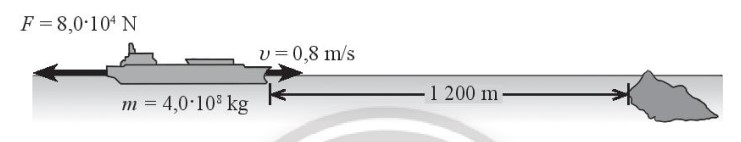
\includegraphics[width=0.7\linewidth]{../figs/VN10-2023-PH-TP016-P-1}
\end{center}
\begin{enumerate}[label=\alph*)]
	\item Tàu có va chạm với bãi đá ngầm không? Nếu vụ va chạm xảy ra thì lượng hàng hoá trên tàu có được an toàn không? Biết vỏ tàu có thể chịu được va đập ở tốc độ tối đa $\SI{0.45}{\meter/\second}$.
	\item Lực tối thiểu do động cơ sinh ra phải bằng bao nhiêu để không xảy ra va chạm giữa tàu và bãi đá ngầm?
\end{enumerate}
\hideall{
\begin{enumerate}[label=\alph*)]
	\item Gọi $v$ là vận tốc của tàu ngay trước khi tàu lùi xa bãi đá ngầm.
	\\
	Áp dụng phương trình định luật II Newton:
	$$\vec{a}=\dfrac{\vec{F}}{m}$$
	Chọn trục $Ox$ hướng từ trái sang phải, chiếu phương trình trên lên trục $Ox$:
	$$a=-\dfrac{F}{m}=-\xsi{\dfrac{1}{5000}}{\meter/\second^2}.$$
	Vì $av<0$ nên tàu chuyển động thẳng chậm dần đều. Gọi $v_s$ là vận tốc của tàu khi đến bãi đá ngầm, ta có $v^2-v^2_s=2as\Leftrightarrow v_s=\sqrt{2as+v^2}=\SI{0.4}{\meter/\second}.$\\
	Nhận thấy $\SI{0}{\meter/\second}\le v_s=\SI{0.4}{\meter/\second}\le \SI{0.45}{\meter/\second}$ nên tàu có va chạm với bãi đá ngầm nhưng hàng hoá trong tàu vẫn được an toàn.
	\item Lực tối thiểu do động cơ sinh ra để tránh va chạm ứng với tốc độ của tàu khi đến bãi đá ngầm bằng 0:
	$$F=m\cdot a'=m\cdot\dfrac{-v^2}{2s}=-\left(\SI{4E8}{\kilogram}\right)\cdot\dfrac{\left(\SI{0.8}{\meter/\second}\right)^2}{2\cdot\left(\SI{1200}{\meter}\right)}\approx\SI{-10.67E4}{\newton}.$$
\end{enumerate}
}



\end{enumerate}